\section{Resultados}
\label{sec:results}

\subsection{Implementación en Simulink}
\label{sec:simulink}
En la Figura \ref{fig:diagBloques} se presenta el diagrama de bloques del sistema descrito anteriormente. Adicionalmente, en la Figura \ref{fig:diagBloques1} se muestra el diagrama de bloques del subsistema representado en la Figura \ref{fig:diagBloques}

\begin{figure}[ht!]
\centering
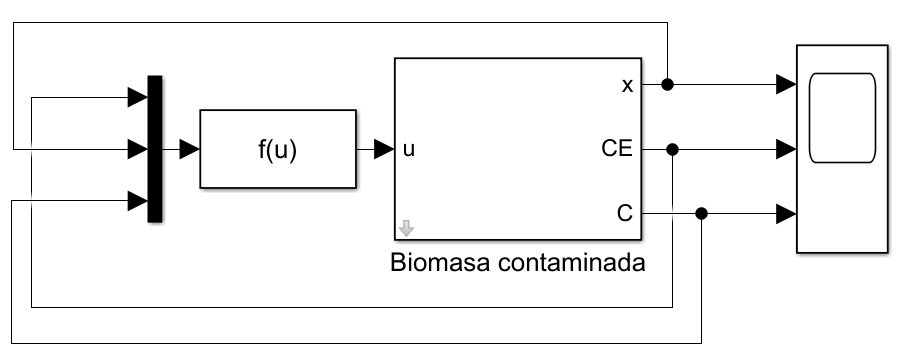
\includegraphics[scale = 0.4]{diagrama-de-bloques1}
\caption{Diagrama de bloques}
\label{fig:diagBloques}
\end{figure}

\subsection{Validación del modelo}
\label{sec:validation}

Siguiendo la guía dada por~\cite{1}, se simuló el sistema utilizando el diagrama de bloques mostrado en la sección~\ref{sec:simulink}. \\
En \cite{1} se define, inicialmente, la siguiente función de control para la entrada:
\begin{equation}
\label{eq:entrada}
u(x, C, C_E) = C_E\left( aX - \frac{bC}{C_E}+ h - \lambda * \ln\left({\frac{C_E}{M}}\right) \right)
\end{equation}
Para la cual es necesario definir los parámetros $M$, que es el límite de la calidad del agua, cantidad de toxina permitida en el ambiente en $\frac{mg}{L}$ y
$\lambda$, un parámetro positivo en $\frac{1}{s}$. \\

Con esta función de estrada realizaremos la validación del modelo, junto con los valores descritos en la Tabla~\ref{tab:validacion}.

\begin{table}[ht!]
\caption{Parámetros para la validación}
\label{tab:validacion}
\centering
\begin{tabular}{|c|c|c|c|c|c|c|c|c|c|c|c|}
\hline
$n$ & $a$ & $b$ & $h$ & $\mu$ & $r_0$ & $K_0$ & $r_1$ & $\rho$ & $M$ & $\lambda$ \\\hline
0.01 & 0.01 & 0.2 & 0.2 & 0.1 & 0.1 & 5 & 0.01 & 2 & 0.5 & 0.01 \\\hline
\end{tabular}
\end{table}

Las condiciones iniciales son:
\begin{itemize}
\item $X(0) = 2mg$
\item $C_E(0) = 2\frac{mg}{L}$
\item $C(0) = 0mg$
\end{itemize}

Los resultados obtenidos por~\cite{1} se muestran en la Figura~\ref{fig:validacion1}. Los resultados para la validación se muestran en la Figura~\ref{fig:validacion2} y en la Figura~\ref{fig:entrada-validacion} se muestra la entrada aplicada al sistema.\\ \ \\
En ambas figuras se observa un comportamiento similar de las tres variables de estado, además de una convergencia a un punto estable similar en ambos casos.

\begin{figure}[ht!]
\centering
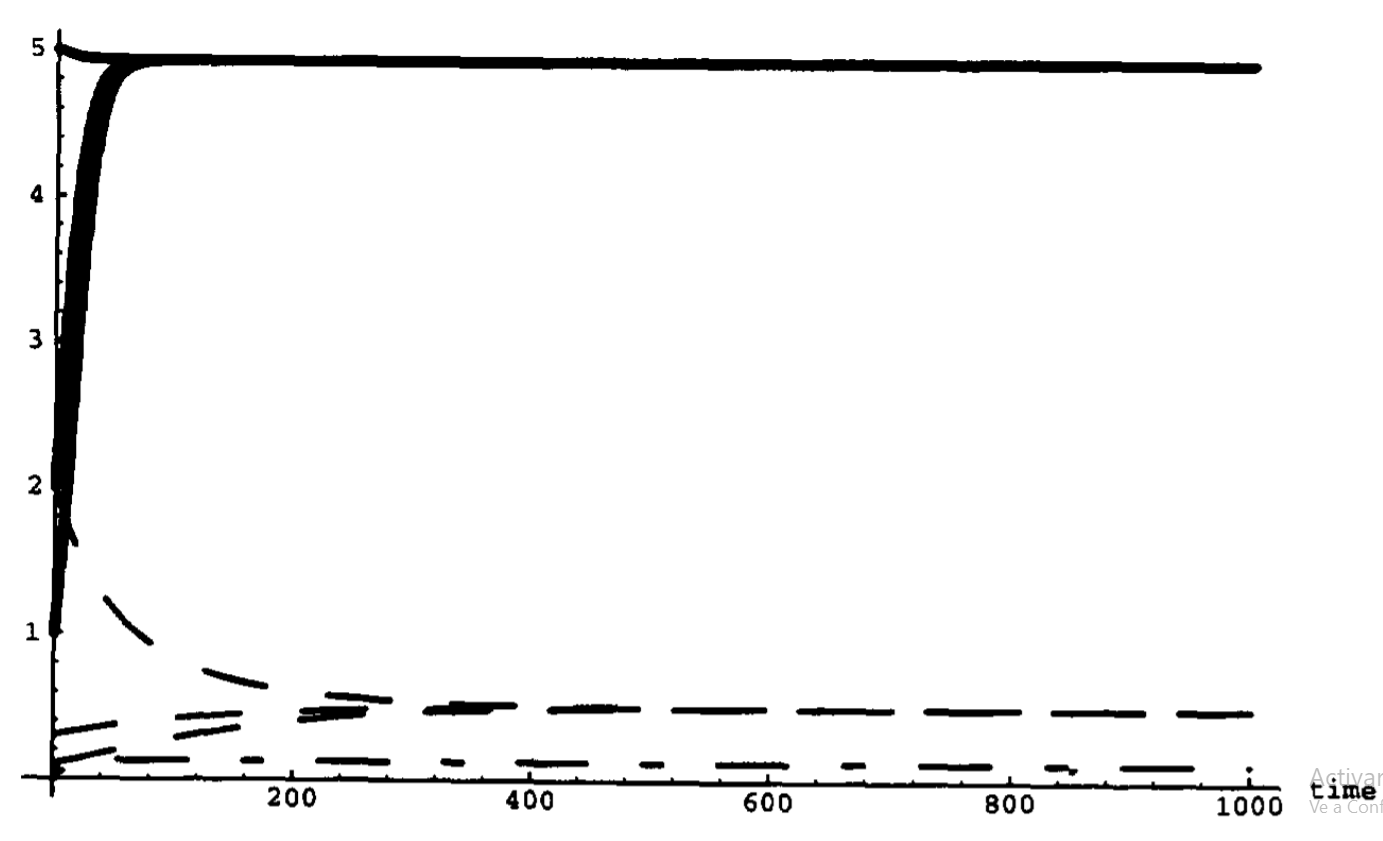
\includegraphics[scale = 0.3]{validacion1}
\caption{Trayectorias para el sistema. Las líneas curvas representan a $X(t)$, las líneas discontinuas representan a $C_E(t)$ y las líneas discontinuas y punteadas representan a $C(t)$. Figura tomada de \cite{1}}
\label{fig:validacion1}
\end{figure}

\begin{figure}[ht!]
\centering
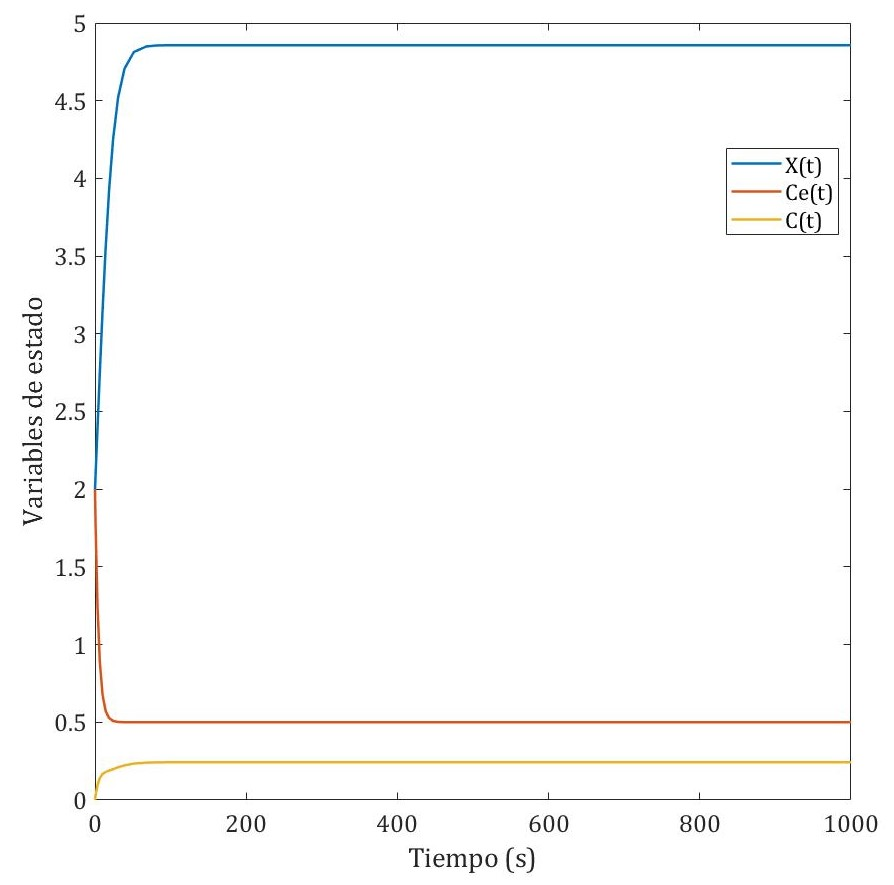
\includegraphics[scale = 0.36]{validacion}
\caption{Resultados del modelo implementado para los valores de los parámetros dados en la Tabla~\ref{tab:validacion}}
\label{fig:validacion2}
\end{figure}
\begin{figure*}[th!]
\centering
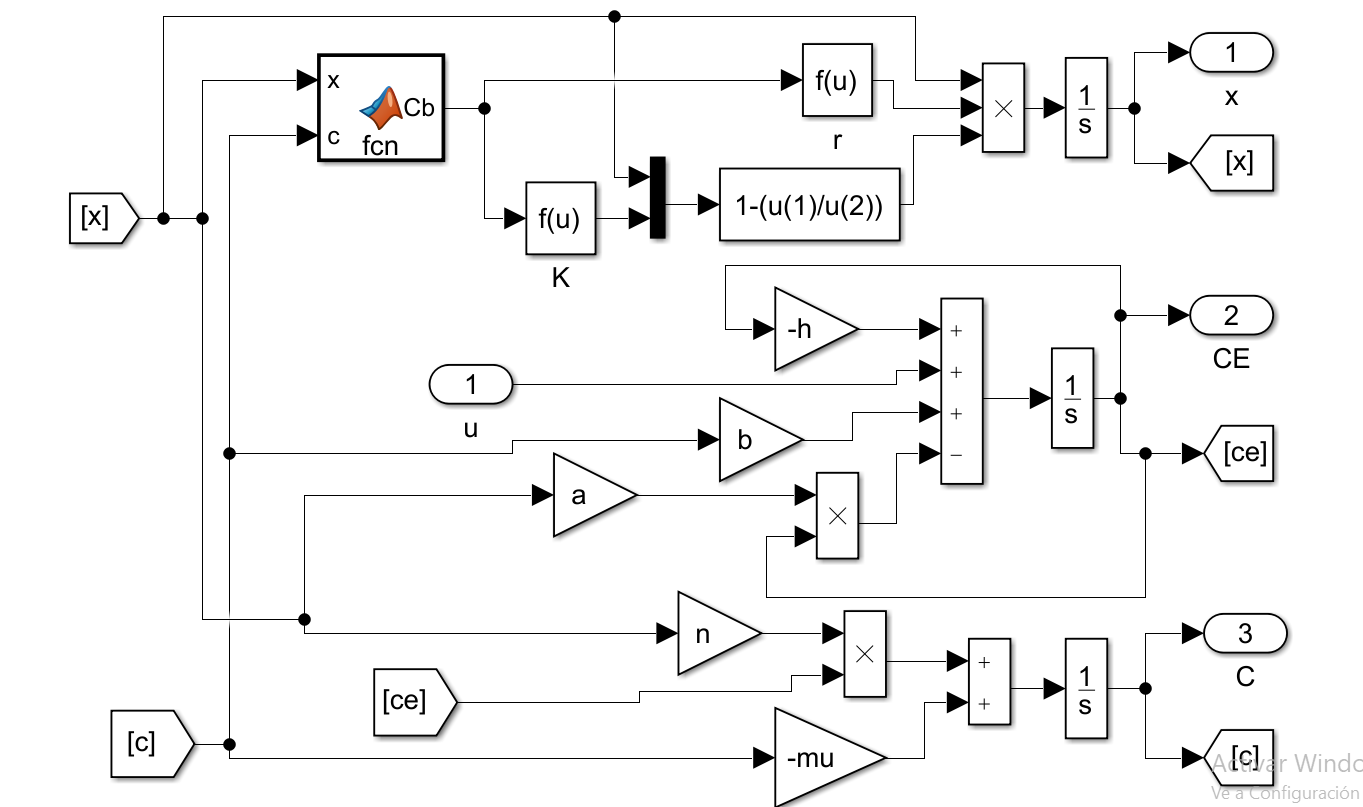
\includegraphics[scale = 0.5]{diagrama-de-bloques}
\caption{Subsistema del diagrama de bloques de la Figura~\ref{fig:diagBloques}}
\label{fig:diagBloques1}
\end{figure*}


\begin{figure}[ht!]
\centering
\includegraphics[scale = 0.36]{entrada-control}
\caption{Entrada del modelo implementado para los valores de los parámetros dados en la Tabla~\ref{tab:validacion}}
\label{fig:entrada-validacion}
\end{figure}

Se hizo, con el propósito de evaluar el impacto de la agregación del parámetro $n$ al modelo, un nuevo experimento en el que se le dio el valor de $n = 0.1\frac{L}{mg*s}$. La gráfica de los resultados de dicho experimento se muestra en la Figura~\ref{fig:validacion-01}. En este, se observa una diferencia significativa en el comportamiento de las variables de estado: los puntos a los que convergen no son los mismos y, $C(t)$, que es la directamente afectada por el parámetro tiene un ascenso mucho más brusco que anteriormente.

\begin{figure}[ht!]
\centering
\includegraphics[scale = 0.36]{validacion-01}
\caption{Resultados del modelo para el cambio del parámetro $n$ y los valores de los parámetros en la Tabla~\ref{tab:validacion}}
\label{fig:validacion-01}
\end{figure}

\subsection{Simulación con diferentes tipos de entrada}
\label{sec:inputs}
Para estos experimentos, se tendrán en cuenta los parámetros descritos en la Tabla~\ref{tab:validacion}. Adicionalmente, al sistema le fue introducido un ruido blanco aleatorio de potencia $0.0005$ que indica un error en la medición final de las variables y se modificó el tiempo de simulación para que fuese $200s$. \\
Dado que los resultados presentados en la Figura~\ref{fig:validacion2} tienen como entrada un sistema de control, en la Figura se muestra una simulación de $200s$ con una entrada constante de $0.12\frac{mg}{L*s}$, para tener una referencia del comportamiento del sistema con el valor de los parámetros. Dicha simulación se muestra en la Figura~\ref{fig:entrada-constante} \\
\begin{figure}[th!]
\centering
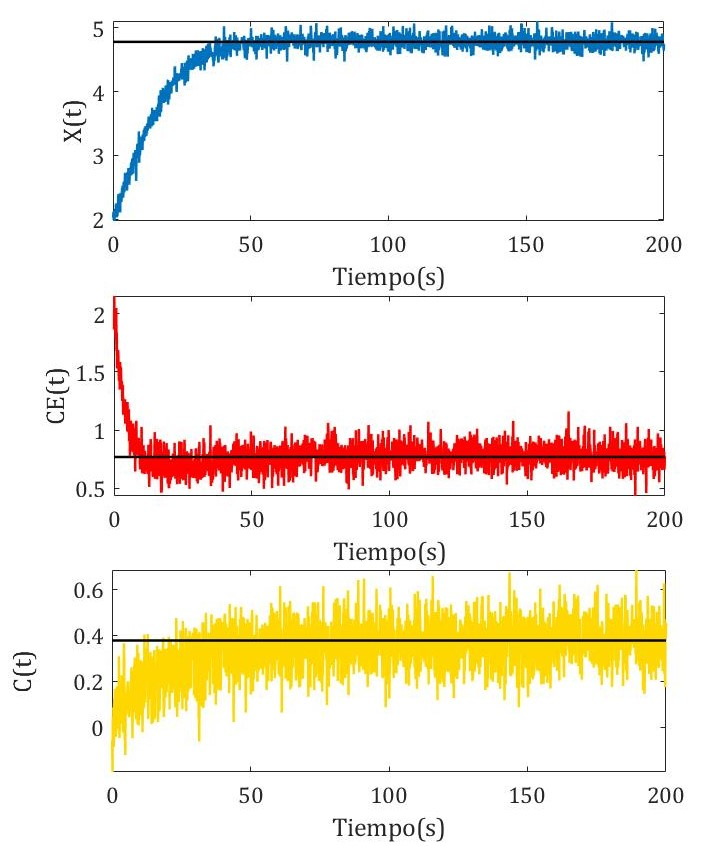
\includegraphics[scale = 0.4]{entrada-constante1}
\caption{Resultados del modelo con entrada constante y ruido}
\label{fig:entrada-constante}
\end{figure}
Se observa un comportamiento similar al de la simulación con controlador: la biomasa de la población $X(t)$ se estabiliza cerca de los $4.7mg$, $C_E(T)$ desciende hasta estabilizarse alrededor de $0.8\frac{mg}{L}$ y $C(t)$ es ascendente al inicio y se estabiliza en un valor cercano a los $0.4mg$. \\ \ \\
Ahora, veremos qué sucede en el sistema al aplicarle diferentes tipos de entrada:
\begin{enumerate}
\item \textbf{Escalón:} Una entrada escalón de $0.5\frac{mg}{L*s}$ en el tiempo $t = 50s$ fue introducida al sistema produciendo los resultados que se muestran en la Figura~\ref{fig:entrada-escalon}. \\
Como se muestra, la biomasa de la población $X(t)$ es creciente hasta aproximadamente el tiempo $t = 50s$, mientras que $C_E(t)$ y $C(t)$ son decrecientes. Posterior a ese tiempo, la biomasa empieza a descender para estabilizarse en un valor alrededor de los $4.2mg$, $C_E(t)$ en $3\frac{mg}{L}$ y $C(t)$ en $1.4mg$ \\

\begin{figure}[ht!]
\centering
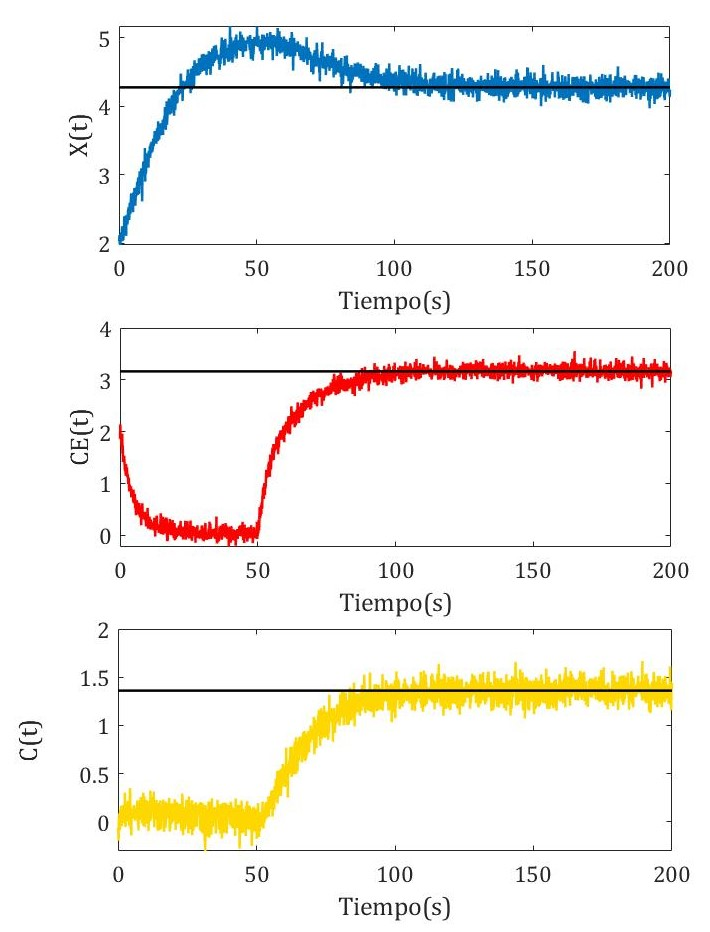
\includegraphics[scale = 0.4]{entrada-escalon}
\caption{Resultados del modelo con entrada escalón en $t = 50$ y ruido}
\label{fig:entrada-escalon}
\end{figure}

\item \textbf{Escalera:} Una entrada escalera como la que se muestra en la Figura~\ref{fig:entrada-escalera1} es introducida al sistema produciendo una salida como la que se muestra en la Figura~\ref{fig:entrada-escalera}. \\
Esta entrada, significa que cada $20s$, es introducido al sistema $0.1\frac{mg}{L*s}$ de toxina más de lo que se le había ingresado
En las gráficas de salida de las variables de estado se nota que, al inicio de la simulación $X(t)$ tiende a crecer, $C_E(t)$ a decrecer igual que $C(t)$, que es el comportamiento esperado para una entrada de $0\frac{mg}{L*s}$ de toxina. Sin embargo, a medida que la entrada aumenta, $X(t)$ llega a un pico cerca de $4.7mg$ cerca del tiempo $t = 40s$, dos pulsos después, y empieza a disminuir de manera abrupta. En sentido contrario, $C_E(t)$ baja bruscamente en los primeros periodos de tiempo, y alrededor de $t = 20s$ comienza a ascender respondiendo a la entrada de toxina en cada uno de los periodos de tiempo. No se observa que llegue a estabilizarse en algún punto. Este comportamiento es similar al que presenta $C(t)$, que comienza a subir alrededor de $t = 30s$ y no parece estabilizarse en ningún valor.

\begin{figure}[th!]
\centering
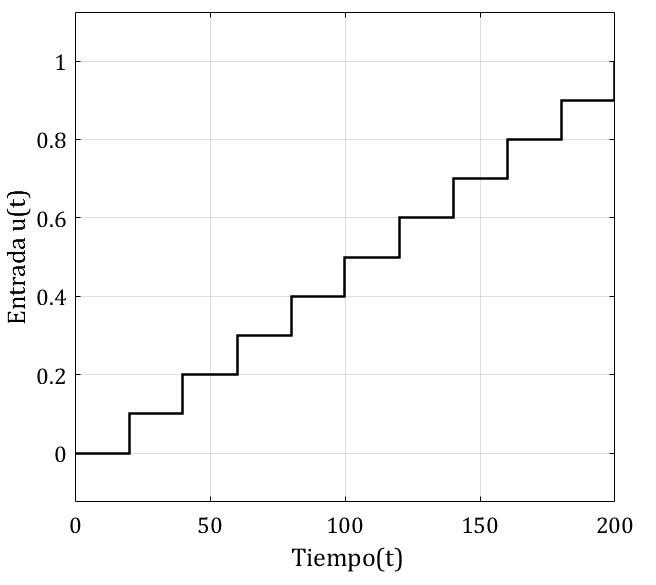
\includegraphics[scale = 0.4]{entrada-escalera1}
\caption{Entrada escalera con paso $t = 20s$ y cambio $0.1\frac{mg}{L*s}$}
\label{fig:entrada-escalera1}
\end{figure}

\begin{figure}[th!]
\centering
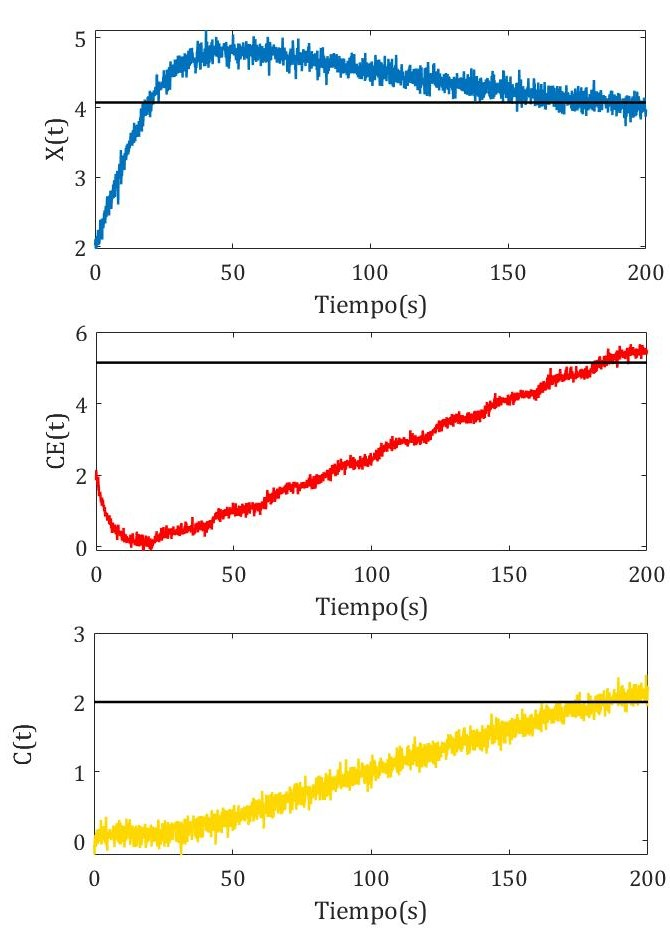
\includegraphics[scale = 0.4]{entrada-escalera}
\caption{Resultados del modelo con entrada escalera mostrada en la Figura~\ref{fig:entrada-escalera1} y ruido}
\label{fig:entrada-escalera}
\end{figure}

\item \textbf{Seno:} Se aplicó una entrada seno como se muestra en la Figura~\ref{fig:entrada-seno}, con amplitud $0.5$ y frecuencia $0.2Hz$. Esta entrada, aunque no tiene significado físico, pues no es posible ingresar toxina en una onda sinusoidal al sistema, nos permitirá observar el comportamiento del mismo. Si quisiéramos darle algún sentido, los valores positivos del seno indican el momento en que se ingresa toxina al sistema y los negativos el momento de sustracción de toxina. En cada una de las gráficas, en morado, se puede observar la entrada que fue aplicada al sistema.

\begin{figure}[ht]
\centering
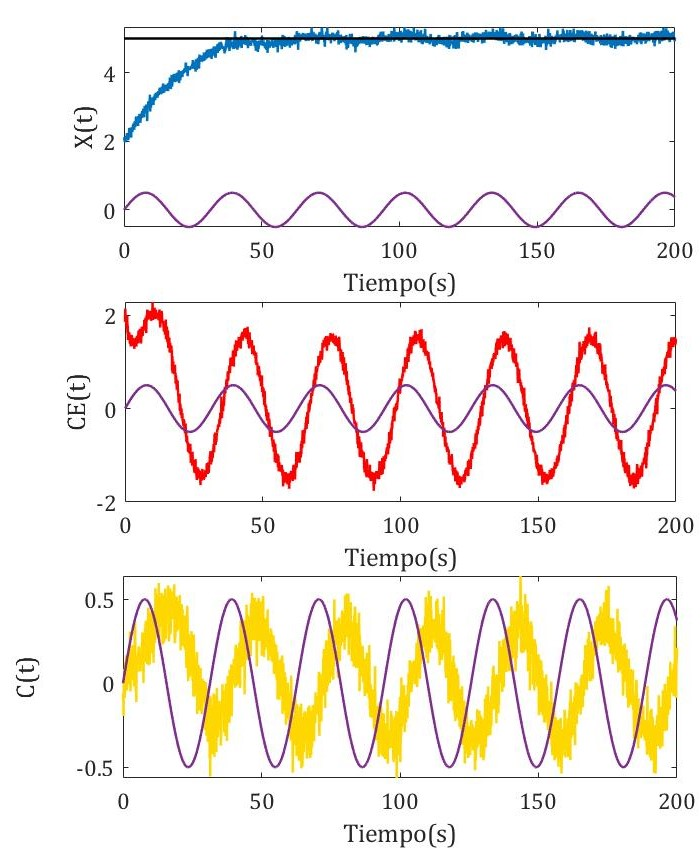
\includegraphics[scale = 0.4]{entrada-seno}
\caption{Resultados del modelo con entrada seno (morado) y ruido}
\label{fig:entrada-seno}
\end{figure}

Podemos observar que $X(t)$, presenta ligeras oscilaciones alrededor de un punto cercano a $4.8mg$. Sin embargo, las otras variables de estado presentan mucha fluctuación. $C_E(t)$ toma valores entre $-1.8\frac{mg}{L}$ y $1.8\frac{mg}{L}$ y $C(t)$ toma valores entre $-0.5mg$ y $0.5mg$.
\end{enumerate}


\subsection{Cambio en los parámetros}
\label{sec:parameters}
Observaremos. el efecto que tiene sobre el sistema hacer cambios en dos de los parámetros, escogidos arbitrariamente. La entrada considerada para estos experimentos es una constante de valor $0.12\frac{mg}{L*s}$\\

\subsubsection{Cambio en la capacidad de carga}
Con respecto a los parámetros considerados en la Tabla~\ref{tab:validacion}, se hará un cambio en la capacidad de carga del sistema en ausencia de toxina, $K_0$, que antes era 5, será aumentada con incrementos de 1 hasta alcanzar 10. En la Tabla~\ref{tab:cambio-par1} se muestran los resultados de las simulaciones realizadas. A modo de notación, nos referiremos a $M(X(t))$, $M(C_E(t))$ y $M(C(t))$ como el valor medio en el que se ve que se estabiliza cada una de las variables de estado en el largo plazo. Adicionalmente, se muestra en la Figura~\ref{fig:cambio-par1} tres de los cambios hechos y cómo se comporta cada una de las variables de estado ante esos cambios.

\begin{table}[ht!]
\centering
\caption{Cambio en la capacidad de carga $K_0$}
\label{tab:cambio-par1}
\begin{tabular}{|c|c|c|c|}
\hline
$K_0$ & $M(X(t))(mg)$ & $M(C_E(t))(\frac{mg}{L})$ & $M(C(t))(mg)$ \\\hline
6 & 5.69 & 0.82 & 0.47 \\\hline
7 & 6.58 & 0.87 & 0.59 \\\hline
8 & 7.47 & 0.94 & 0.71 \\\hline
9 & 8.34 & 1.00 & 0.85 \\\hline
10 & 9.20 & 1.09 & 1.02 \\\hline
\end{tabular}
\end{table}

Al observar la Figura~\ref{fig:cambio-par1}, se puede notar que el punto de estabilización de cada una de las variables de estado es cada vez más alto, a medida que la capacidad de carga del sistema aumenta.

\begin{figure}[ht!]
\centering
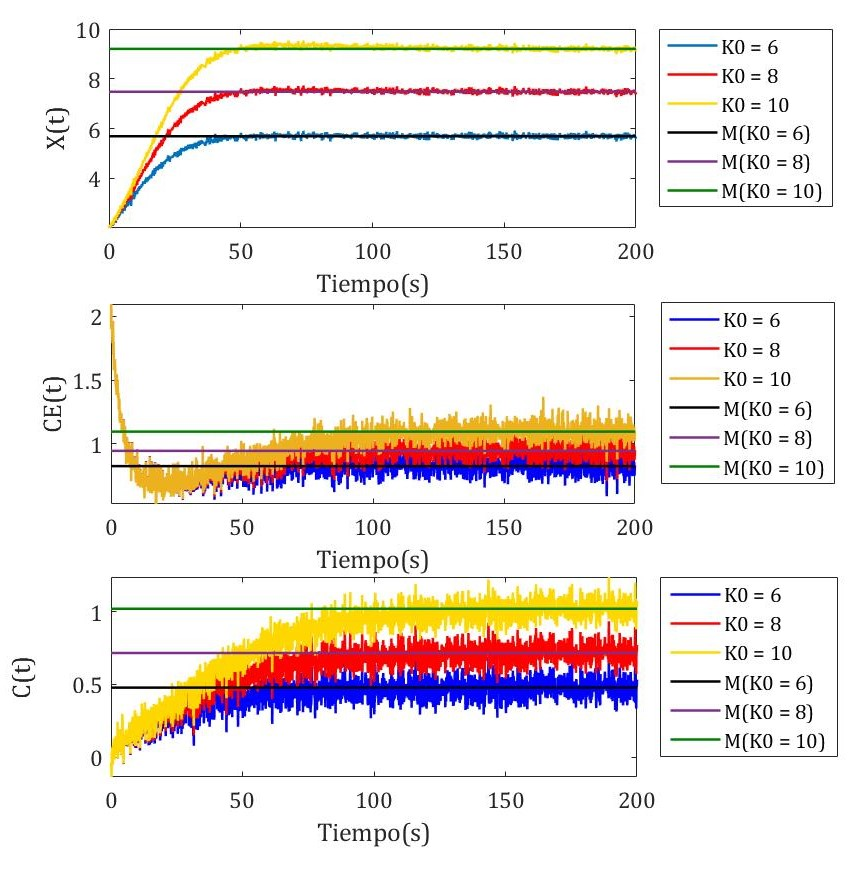
\includegraphics[scale = 0.37]{cambio1}
\caption{Resultados de la simulación para el cambio de $K_0$ con tres valores}
\label{fig:cambio-par1}
\end{figure}

\subsubsection{Cambio en la tasa de eliminación del contaminante por parte del ambiente h}
De igual manera, se consideran los mismos parámetros de la Tabla~\ref{tab:validacion}, y se cambiará el parámetro $h$ para llevarlo de $0.3$ a $0.7$ con un incremento de $0.1$, tal y como se muestra en la Tabla~\ref{tab:cambio-par2}, junto con los resultados de la simulación de cada uno de estos parámetros. De igual manera, se puede observar en la Figura~\ref{fig:cambio-par2} las gráficas para la simulación de 3 de estos valores.
\begin{table}[ht!]
\centering
\caption{Cambio en la tasa de eliminación por parte del ambiente $h$}
\label{tab:cambio-par2}
\begin{tabular}{|c|c|c|c|}
\hline
$h$ & $M(X(t))(mg)$ & $M(C_E(t))(\frac{mg}{L})$ & $M(C(t))(mg)$ \\\hline
0.3 & 4.86 & 0.46 & 0.23 \\\hline
0.4 & 4.90 & 0.32 & 0.16 \\\hline
0.5 & 4.92 & 0.25 & 0.13 \\\hline
0.6 & 4.93 & 0.20 & 0.10 \\\hline
0.7 & 4.94 & 0.17 & 0.09 \\\hline
\end{tabular}
\end{table}

\begin{figure}[ht!]
\centering
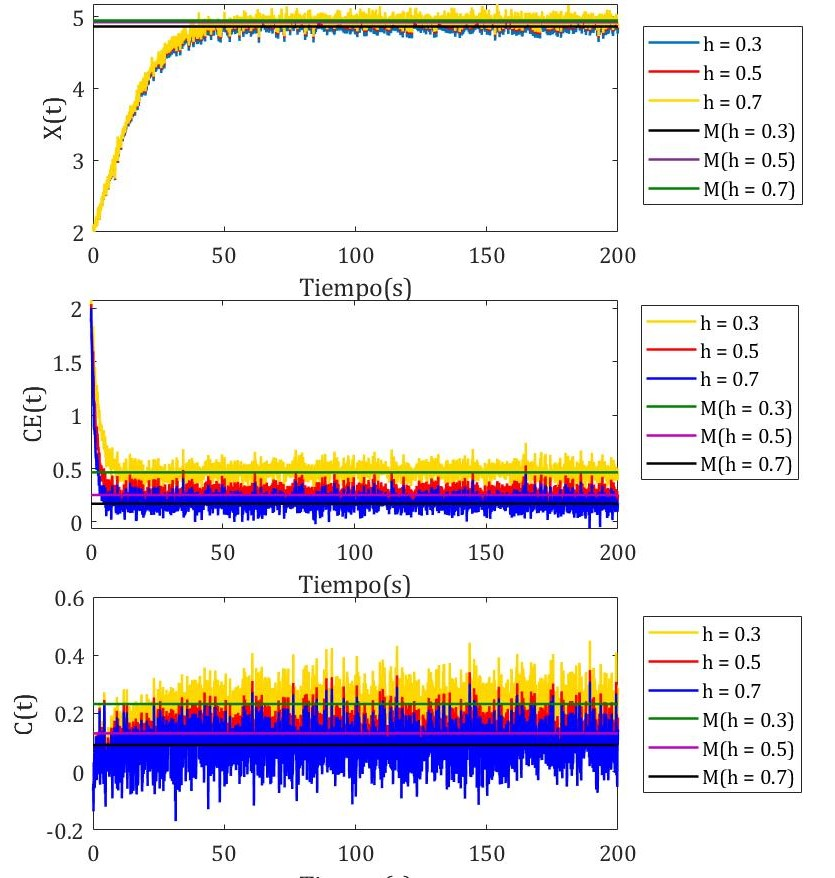
\includegraphics[scale = 0.37]{cambio2}
\caption{Resultados de la simulación para el cambio de $h$ con tres valores}
\label{fig:cambio-par2}
\end{figure}

En la gráfica presentada en la Figura~\ref{fig:cambio-par2}, se puede observar que $X(t)$ está limitada alrededor del mismo valor en todas las simulaciones, mientas que, a medida que la tasa de eliminación aumenta, $C_E(t)$ se estabiliza en valores más bajos, igual que $C(t)$.


\subsection{Solución numérica}
\label{sec:numericos}
Para comparar la solución otorgada por la herramienta de simulación con otros métodos numéricos conocidos, se realizó la implementación en MATLAB de los métodos de Runge-Kutta de orden 4 y Euler para la solución de un sistema de 3 ecuaciones diferenciales de orden 1. \\
Se consideraron, para ello, diferentes tamaños de paso $s$. Sin embargo, no se muestran en esta sección los resultados para valores de $s$ inferiores a $0.7$, puesto que las soluciones son casi idénticas, y no se distingue una de otra. Es interesante ver el caso en el que el paso $s$ para ambos métodos numéricos es $1$, y se muestra en la Figura~\ref{fig:numerico}. El método de Euler empieza a alejarse de la solución proporcionada por Simulink, igual que el de Runge Kutta, sin embargo, este último se mantiene más estable.

\begin{figure}[ht!]
\centering
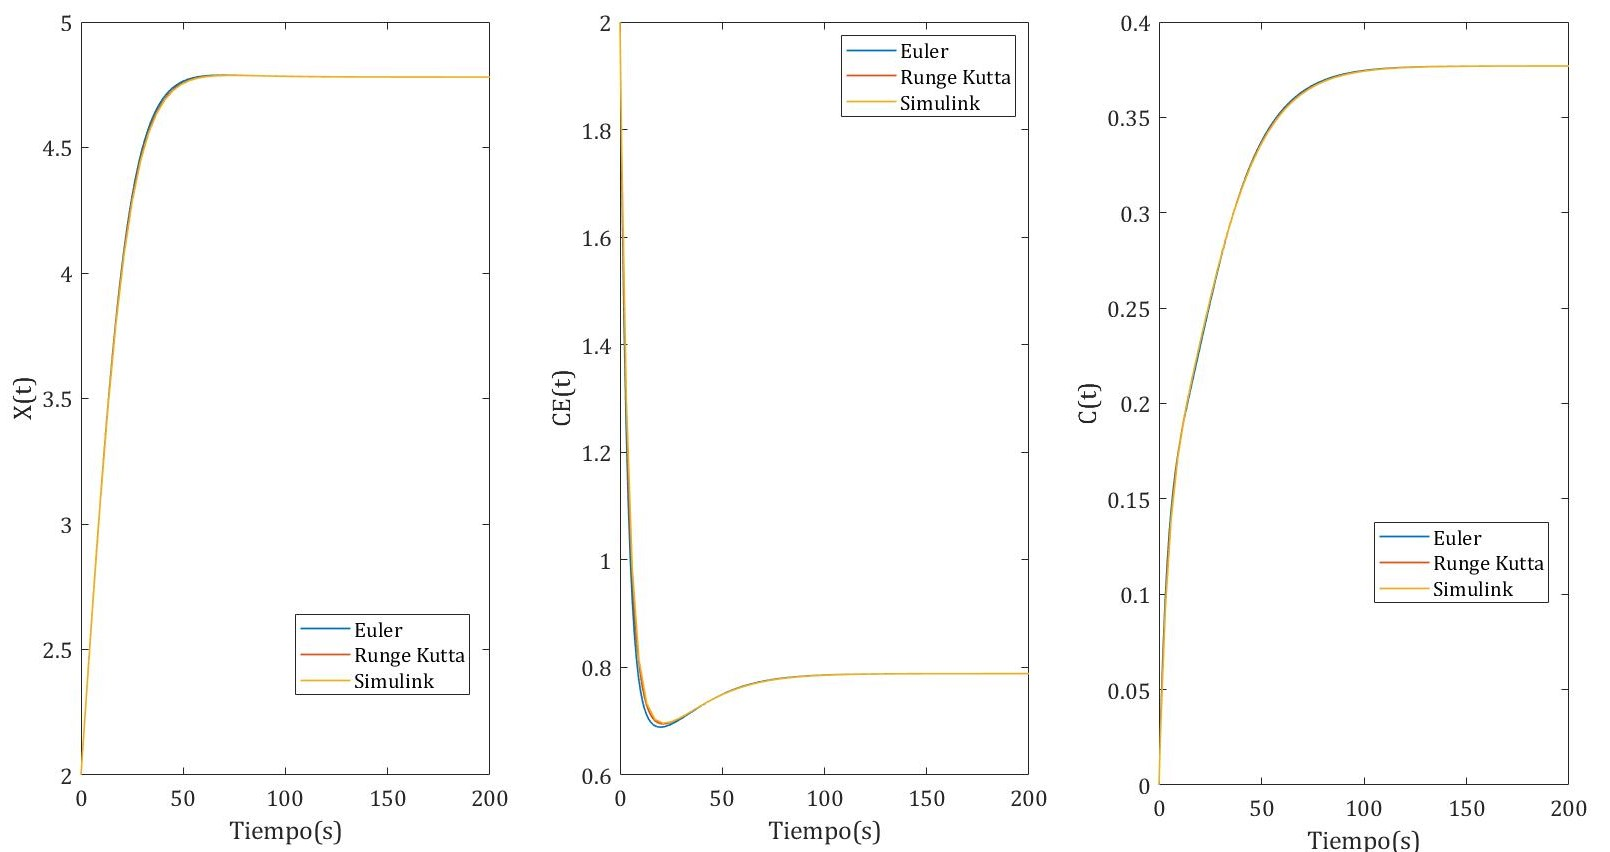
\includegraphics[scale = 0.37]{num1}
\caption{Comparación entre las soluciones del sistema de ecuaciones diferenciales del modelo}
\label{fig:numerico}
\end{figure}

\subsection{Curva de linealidad}
En la Figura~\ref{fig:curva_linealidad} se observa la curva de linealidad para el sistema. La curva roja es la salida $x(t)$, con diferentes entradas. La línea negra representa la línea que aproxima la curva en el punto de operación
[ \vb*{x0} =
  \begin{pmatrix}
    2.9\\
    6.8\\
    23.4
  \end{pmatrix}
\begin{figure}
    \centering
    \includegraphics[scale = 0.4]{cdelinealidad.jpg}
    \caption{Curva de linealidad para la salida del sistema.}
    \label{fig:curva_linealidad}
\end{figure}
